
%
%	Section 2
%

\section{Super-Kamiokande}\label{Section_002}
\Headerfooter{Super-Kamiokande}

\subsection{Super-Kamiokande}
\vs\hs The Super-Kamiokande (SK)~\cite{2003Fukuda} is the experiment held in Kamioka, Gifu, Japan, with the large water Cherenkov detector placed in 1,000 m underground, 2,700 m water equivalent overburden.
The overview of the SK detector is shown in Figure~\ref{002_F01_SK}.
The SK stands for ``Super-Kamioka Neutrino Detection Experiment'' and ``Super-Kamioka Nucleon Decay Experiment''.
The rate of cosmic ray muon is reduced by a factor of 10$^{\text{5}}$ compared to that of the ground level.\\

\begin{figure}[h]
	\centering
	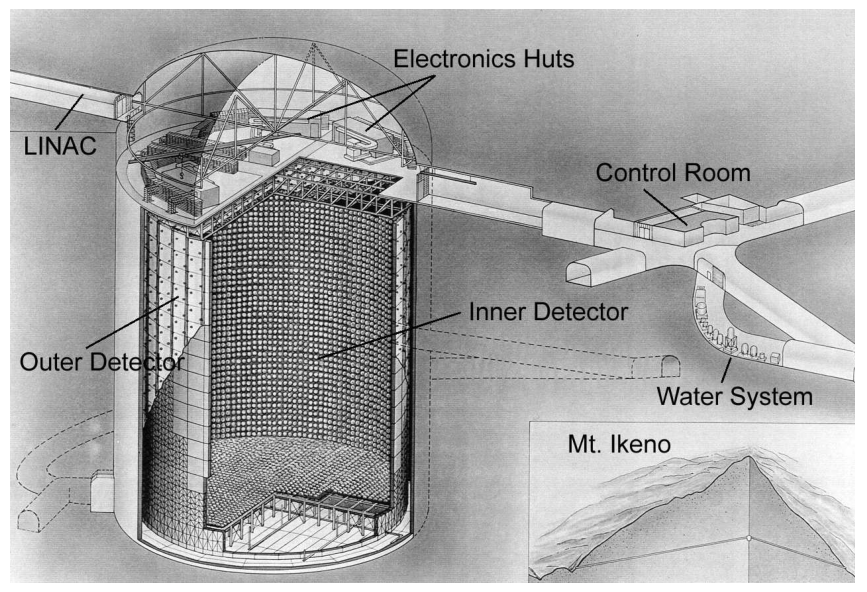
\includegraphics[width=15cm]{Figures/002/F01_SK}
	\caption[Overview of the Super-Kamiokande detector]{\label{002_F01_SK} Overview of the SK detector~\cite{2003Fukuda}.}
\end{figure}

\hs The SK detector consists of the stainless-steel cylindrical tank with a diameter of 39.3 m and a height of 41.4 m and 50 kilotons ultrapure water.
The tank is separated into the inner detector (ID) and the outer detector (OD) by stainless-steel frames (supermodule frames).
The cross section of the SK detector and the overview of supermodule frames are shown in Figure~\ref{002_F02_SK_SM}.
The diameter of ID, the height of ID and the volume of ID (the fiducial volume) is 33.8 m, 36.2 m and 32 kilotons (22.5 kilotons), respectively.
In ID, 11,129 20-inch (50 cm) photomultiplier tubes (PMTs) are installed.
The gaps between ID PMTs are covered by black polyethylene terephthalate sheets.
The sheets separate ID and OD optically and suppress the reflection at the surface of the ID wall.
Moreover, the sheets reduce low energy events by radioactive backgrounds occurring behind the PMTs.
On the other hand, in OD, 1,885 8-inch (20 cm) PMTs are installed.
OD volume is covered by white Tyvek sheets manufactured by DuPont.
The Tyvek sheets have high reflectivity and enhance the light collection efficiency in OD.

\begin{figure}[tbp]
	\centering
	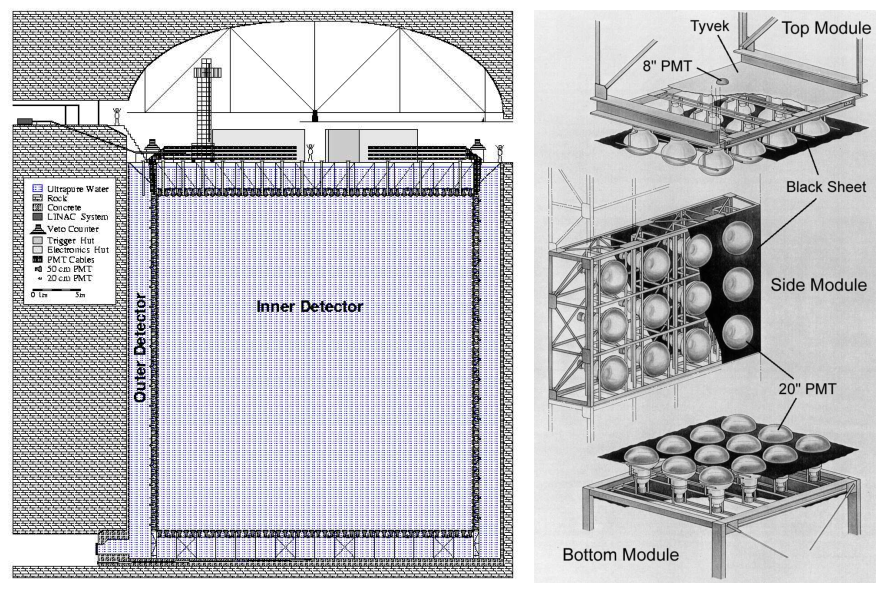
\includegraphics[width=15cm]{Figures/002/F02_SK_SM}
	\caption[Cross section of the SK detector and overview of supermodule frames]{\label{002_F02_SK_SM} Cross section of the SK detector (left) and overview of supermodule frames (right)~\cite{2003Fukuda}.}
\end{figure}

\subsection{ID PMT}
\vs\hs The schematic view of the ID PMT is shown in Figure~\ref{002_F03_IDPMT}.
The number of ID PMTs is 7,650 on the barrel (side walls), 1,740 on the top and 1,739 on the bottom, thus the effective photocathode coverage of ID is 40\%.
The role of ID PMTs is to reconstruct the energy, generated position, direction and the kind of the charged particles.
Figure~\ref{002_F04_IDPMTQE} shows the quantum efficiency of the ID PMT photocathode as a function of wavelength.
The material of photocathode is bialkali (Sb-K-Cs) and the quantum efficiency is about 21\% at 360 - 400 nm.
Figure~\ref{002_F05_IDPMT1pe} shows the single photoelectron pulse height distribution of the ID PMT.
The peak around zero ADC count is caused by PMT dark current.
Figure~\ref{002_F06_IDPMTt} shows the relative transit time distribution for a typical ID PMT tested using 410 nm wavelength light at the single photoelectron intensity level.
The 1$\sigma$ of transit time for a single photoelectron signal is 2.16 ns.

\begin{figure}[tbp]
	\centering
	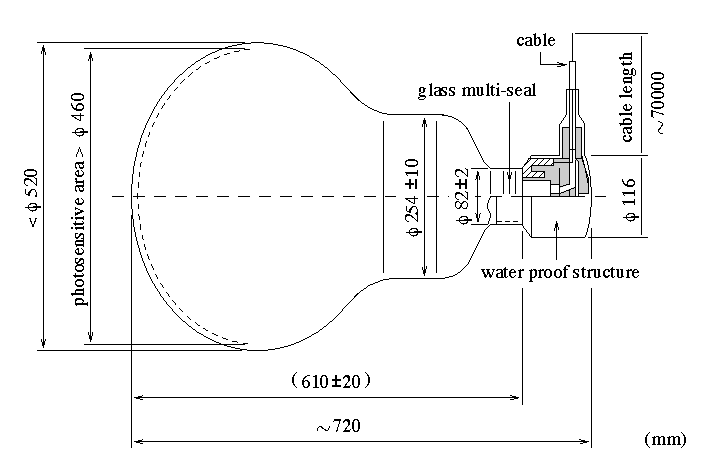
\includegraphics[width=12cm]{Figures/002/F03_IDPMT}
	\caption[Schematic view of the ID PMT]{\label{002_F03_IDPMT} Schematic view of the ID PMT~\cite{2003Fukuda}.}
\end{figure}

\begin{figure}[tbp]
	\centering
	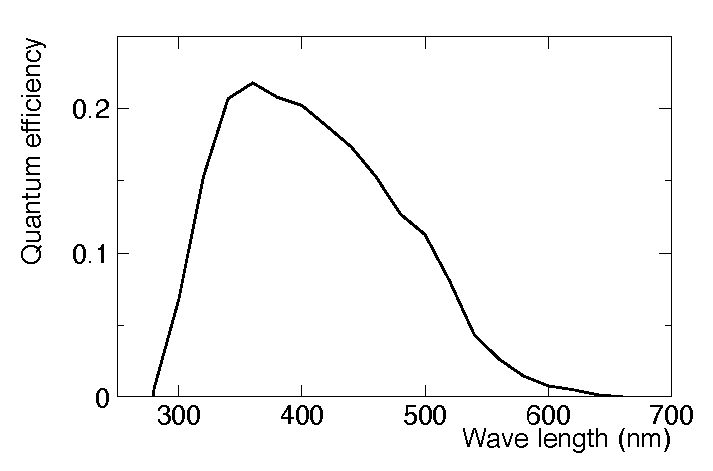
\includegraphics[width=12cm]{Figures/002/F04_IDPMTQE}
	\caption[Quantum efficiency of the ID PMT photocathode as a function of wavelength]{\label{002_F04_IDPMTQE} Quantum efficiency of the ID PMT photocathode as a function of wavelength~\cite{2003Fukuda}. The material of ID PMT photocathode is bialkali (Sb-K-Cs).}
\end{figure}

\begin{figure}[tbp]
	\centering
	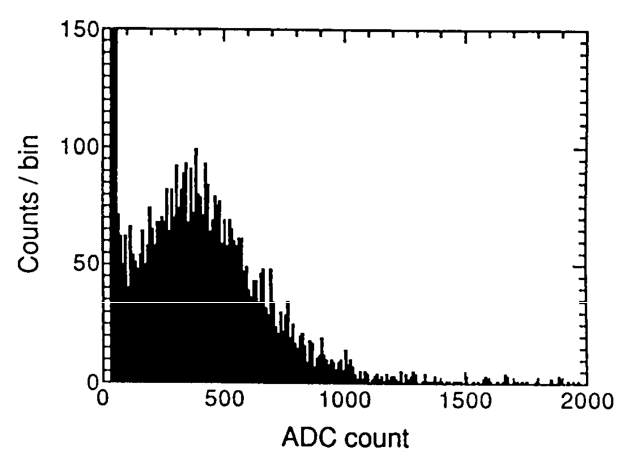
\includegraphics[width=12cm]{Figures/002/F05_IDPMT1pe}
	\caption[Single photoelectron pulse height distribution of the ID PMT]{\label{002_F05_IDPMT1pe} Single photoelectron pulse height distribution of the ID PMT~\cite{2003Fukuda}. The peak around zero ADC count is caused by PMT dark current.}
\end{figure}

\begin{figure}[tbp]
	\centering
	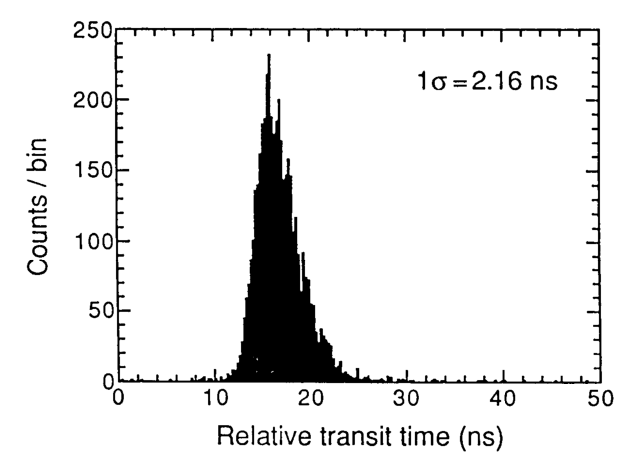
\includegraphics[width=12cm]{Figures/002/F06_IDPMTt}
	\caption[Relative transit time distribution for a typical ID PMT tested using 410 nm wavelength light at the single photoelectron intensity level]{\label{002_F06_IDPMTt} Relative transit time distribution for a typical ID PMT tested using 410 nm wavelength light at the single photoelectron intensity level~\cite{2003Fukuda}.}
\end{figure}

\subsection{OD PMT}
\vs\hs The number of OD PMTs is 1,275 on the barrel, 302 on the top and 308 on the bottom.
To compensate the small number of OD PMTs, wavelength shifting (WS) plate is attached to each OD PMT.
The WS plate is square acrylic panel with a side of 60 cm and a thickness of 1.3 cm, doped with 50 mg$/$L of bis-MSB (C$_{\text{24}}$H$_{\text{22}}$).
The WS plate absorbs UV light, and then emit photons in the blue - green.
OD PMT with bialkali photocathode is more sensitive to blue - green photons than UV photons.
Therefore, the light collection efficiency is improved by about a factor of 1.5 compared to without WS plates.
The timing resolution of OD PMTs with WS plates is 15 ns (FWHM), which is poorer than that of ID PMTs.
However, OD was optimized as a veto counter and the poorer timing resolution is less important.
Figure~\ref{002_F07_IDODPMT} shows the positional relationship of ID PMTs and OD PMTs in a supermodule frame.
Basically, in a supermodule frame, 12 ID PMTs and 2 OD PMTs are attached.

\begin{figure}[h]
	\centering
	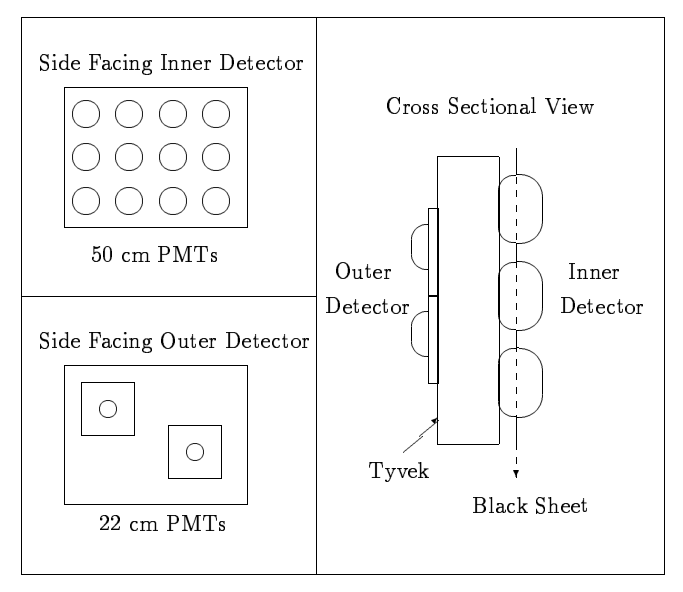
\includegraphics[width=10cm]{Figures/002/F07_IDODPMT}
	\caption[Positional relationship of ID PMTs and OD PMTs in a supermodule frame]{\label{002_F07_IDODPMT} Positional relationship of ID PMTs and OD PMTs in a supermodule frame~\cite{1997ZoaPhD}. 12 ID PMTs and 2 OD PMTs are attached in a supermodule frame, basically.}
\end{figure}

\subsection{Helmholtz coils}
\vs\hs The geomagnetic field would affect photoelectron trajectories and timing in the PMTs.
Therefore, 26 sets of horizontal and vertical Helmholtz coils are deployed around the inner surface of the tank to reduce the geomagnetic field.
Figure~\ref{002_F08_Coil} shows the schematic view of Helmholtz coils.
The average geomagnetic field intensity without Helmholtz coils is about 450 mG~\cite{2003Fukuda}.
The average field intensity can be reduced to 32 mG with Helmholtz coils, resulting that the deviation in the collection efficiency of photoelectrons is 2\%~\cite{2014AbeCalib}.

\begin{figure}[tbp]
	\centering
	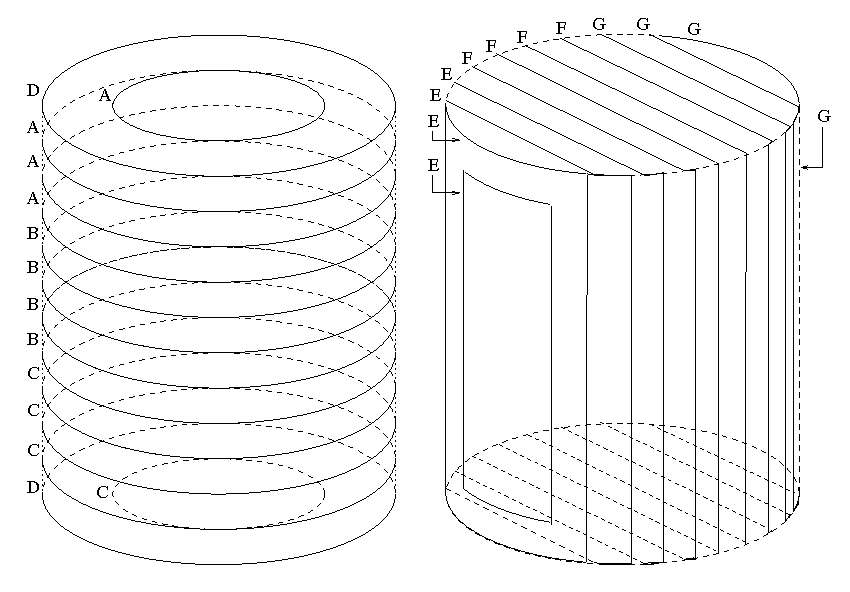
\includegraphics[width=12cm]{Figures/002/F08_Coil}
	\caption[Schematic view of Helmholtz coils]{\label{002_F08_Coil} Schematic view of Helmholtz coils~\cite{1998YamaguchiPhD}.}
\end{figure}

\subsection{Observation phase}\label{002_Obs_pha}
\vs\hs The observation phase of SK is categorized into seven, from SK-I to SK-VII.
Each observation phase is described below.\\
\\
\textbf{SK-I}\\
\hs SK-I started in April 1996 and ended in July 2001.
In ID, 11,146 PMTs were attached and the effective photocathode coverage of ID was 40\%.
It was during the SK-I that we got the evidence for neutrino oscillation~\cite{1998Fukuda}.\\
\\
\textbf{SK-II}\\
\hs In November 12th, 2001, one bottom PMT broke when ultrapure water was filled into SK detector after finishing the detector maintenance.
Due to the shockwave generated at that time, other PMTs were broken in a chain.
As a result, it became a serious accident that 6,779 ID PMTs and 1,017 OD PMTs were lost.
In SK-II, which started in October 2002 and ended in October 2005, the observation was performed using 5,182 remained and spare ID PMTs and 1,885 remained and new OD PMTs.
The effective photocathode coverage of ID was 19\%.
Since SK-II, each ID PMT has been covered with a shockwave prevention case.
The case consists of an acrylic that covers the photocathode and Fiber Reinforced Plastic (FRP) case that covers parts other than the photocathode.
The case not only prevents shockwave but also increases the water pressure resistance of the PMT.
The picture of a shockwave prevention case is shown in Figure~\ref{002_F09_Case}.\\

\begin{figure}[tbp]
	\centering
	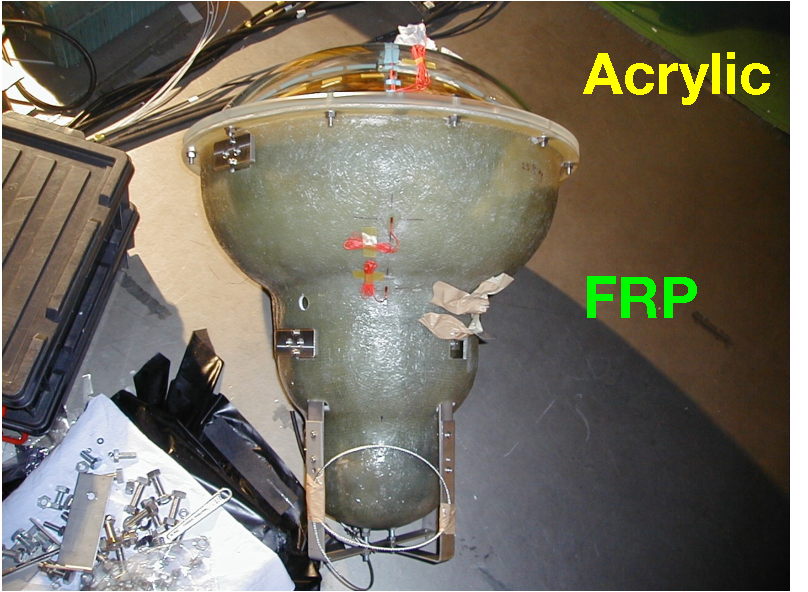
\includegraphics[width=8cm]{Figures/002/F09_Case}
	\caption[Picture of a shockwave prevention case]{\label{002_F09_Case} Picture of a shockwave prevention case~\cite{SKaccident}.}
\end{figure}

\textbf{SK-III}\\
\hs SK-III started in July 2006 and ended in August 2008.
Since SK-III, the number of ID PMTs has been 11,129 and the effective photocathode coverage of ID has been 40\%.
The reason why the number of ID PMTs is reduced by 17 compared to SK-I is that ID PMTs cannot be installed at the edge of the detector because the size of the shockwave prevention case is large.\\
\\
\textbf{SK-IV}\\
\hs In September 2008, the data acquisition system was renewed from Analog Timing Module (ATM) to QTC-Based Electronics with Ethernet (QBEE) and SK-IV started~\cite{2009Nishino}.
QTC stands for charge-to-time converter.
The renewal of the system allows us to open the data acquisition time window until 535 $\mu$s from the trigger timing and enabled to search neutron signals~\cite{2009Watanabe}.
SK-IV continued until June 2018 and is longest phase at this time.\\
\\
\textbf{SK-V}\\
\hs The tank refurbishment work toward the SK-Gd experiment was conducted between SK-IV and SK-V.
The purpose of the work was the water stop reinforcement of the tank, the piping improvement in the tank and the PMT replacement.
After finishing the work, SK-V started in January 2019 and ended in July 2020.\\
\\
\textbf{SK-VI}\\
\hs In July 2020, we dissolved 13.2 tons of Gd$_{\text{2}}$(SO$_{\text{4}}$)$_{\text{3}}\,\cdot\,$8H$_{\text{2}}$O (we introduced 0.011\% of Gd) into the SK tank and SK-VI (the SK-Gd experiment) started.
The time constant of neutron capture at this Gd concentration is about 115 $\mu$s~\cite{2022Abe}.
SK-VI continued until June 2022.\\
\\
\textbf{SK-VII}\\
\hs In June 2022, we additionally dissolved 27.3 tons of Gd$_{\text{2}}$(SO$_{\text{4}}$)$_{\text{3}}\,\cdot\,$8H$_{\text{2}}$O into the SK tank and SK-VII started.
The Gd concentration is comparable to 0.03\%.
The time constant of neutron capture at this Gd concentration is about 62 $\mu$s.\\
\\
\hs The information of each observation phase is summarized in Table~\ref{002_Tab:phase}.

\begin{table}[h]
	\caption[Information of each observation phase]{\label{002_Tab:phase} Information of each observation phase.}
	\centering
	\vs
	\begin{tabular}{lrrr}
		\hline\hline
		Phase&SK-I&SK-II&SK-III\\
		\hline
		Start&Apr. 1996&Oct. 2002&Jul. 2006\\
		End&Jul. 2001&Oct. 2005&Sep. 2008\\
		\# of ID PMTs (Coverage)&11,146 (40\%)&5,182 (19\%)&11,129 (40\%)\\
		\# of OD PMTs&1,885&1,885&1,885\\
		Electronics&ATM&ATM&ATM\\
		Gd concentration&0\%&0\%&0\%\\
		\hline\hline
	\end{tabular}
	\\
	\vs
	\begin{tabular}{lrrrr}
		\hline\hline
		Phase&SK-IV&SK-V&SK-VI&SK-VII\\
		\hline
		Start&Sep. 2008&Jan. 2019&Jul. 2020&Jun. 2022\\
		End&Jun. 2018&Jul. 2020&Jun. 2022&-\\
		\# of ID PMTs (Coverage)&11,129 (40\%)&11,129 (40\%)&11,129 (40\%)&11,129 (40\%)\\
		\# of OD PMTs&1,885&1,885&1,885&1,885\\
		Electronics&QBEE&QBEE&QBEE&QBEE\\
		Gd concentration&0\%&0\%&0.011\%&0.03\%\\
		\hline\hline
	\end{tabular}
\end{table}

\begin{figure}[tbp]
	\centering
	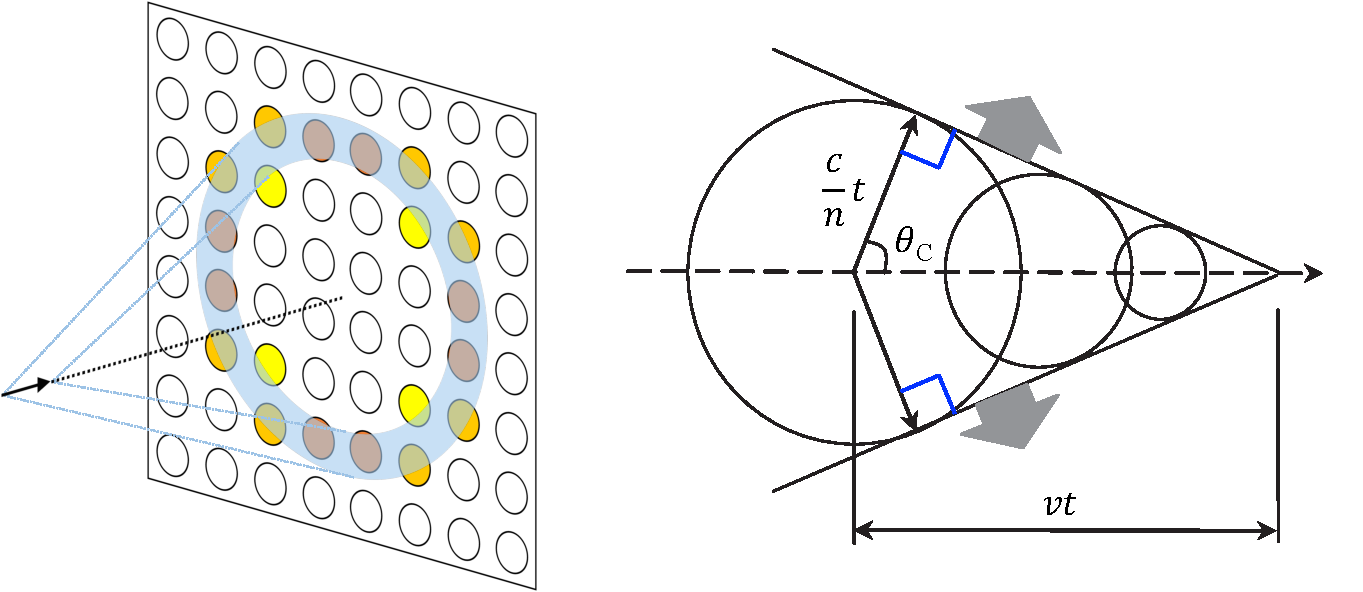
\includegraphics[width=15cm]{Figures/002/F12_Cherenkov}
	\caption[Schematic view of Cherenkov radiation]{\label{002_F12_Cherenkov} Schematic view of Cherenkov radiation~\cite{2015Yamamoto}.}
\end{figure}

\subsection{Detection principle}
\vs\hs When the speed of the charged particle passing through the dielectric medium is faster than the speed of light in the medium, photons are radiated conically along the track of the particle.
This phenomenon is called ``Cherenkov radiation'', and the radiated photons are called ``Cherenkov photons''.
Figure~\ref{002_F12_Cherenkov} shows the schematic view of Cherenkov radiation.
The Cherenkov photons are projected in a ring as shown in left side of Figure~\ref{002_F12_Cherenkov}.
The ring is called ``Cherenkov ring''.
In the SK, the energy, generated position, direction and the kind of the charged particle are reconstructed using the time, quantity of charge and Cherenkov ring pattern information that ID PMTs received.
In right side of Figure~\ref{002_F12_Cherenkov}, the charged particle with velocity $v$ moves distance $vt={v \over c}ct=\beta ct$ in time $t$, where $c$ is the speed of light in vacuum and $\beta={v \over c}$ is the ratio of $v$ and $c$.
While the Cherenkov photon moves distance ${c \over n}t$ in time $t$, where $n$ is the refractive index of the dielectric medium.
Therefore, when the angle between the direction of charged particle and the direction of Cherenkov photon is defined as $\theta_{\text{C}}$, the next formula is established,
\begin{eqnarray}\label{002_Eq_Che}
	\cos\theta_{\text{C}}={{c \over n}t \over \beta ct}={\text{1} \over n\beta}.
\end{eqnarray}
In Equation (\ref{002_Eq_Che}), assuming that $n=\,$1.34, which is the refractive index of water, and $\beta=\,$1, $\theta_{\text{C}}$ becomes about 42$^{\circ}$.
Therefore, in water, the maximum angle between the direction of charged particle and the direction of Cherenkov angle is about 42$^{\circ}$.\\
\hs The energy $E$ required for the charged particle with rest mass $m$ to emit Cherenkov photons (Cherenkov threshold) is
\begin{eqnarray}
	E={mc^{\text{2}} \over \sqrt{\text{1}-\beta^{\text{2}}}}\geq{mc^{\text{2}} \over \sqrt{\text{1}-\Big({\text{1} \over n}\Big)^{\text{2}}}}={nmc^{\text{2}} \over \sqrt{n^{\text{2}}-\text{1}}}.
\end{eqnarray}
The Cherenkov threshold of main charged particles is summarized in Table~\ref{002_Tab:Che}.\\
\hs Assuming that the wavelength region of Cherenkov photons is from $\lambda_{\text{1}}$ to $\lambda_{\text{2}}$, the number of Cherenkov photons $N$ emitted per unit length $x$ when the particle with charge $z$ passes through the medium is
\begin{eqnarray}
	{dN \over dx}=\text{2}\pi\alpha z^{\text{2}}\sin ^{\text{2}} \theta_{\text{C}}\bigg({\text{1} \over \lambda_{\text{1}}}-{\text{1} \over \lambda_{\text{2}}}\bigg),
\end{eqnarray}
where $\alpha$ is the fine-structure constant.

\begin{table}[tbp]
	\caption[Cherenkov threshold of main charged particles]{\label{002_Tab:Che} Cherenkov threshold of main charged particles~\cite{2022Workman}. $m$ is rest mass and $E$ is Cherenkov threshold. Here $n=\,$1.34 is assumed.}
	\centering
	\vs
	\begin{tabular}{lrrrrr}
		\hline\hline
		Charged particle&e$^{\pm}$&$\mu^{\pm}$&$\pi^{\pm}$&K$^{\pm}$&p\\
		\hline
		$m$ [MeV$/c^{\text{2}}$]&0.511&105.658&139.570&493.677&938.272\\
		$E$ [MeV]&0.768&158.730&209.676&741.652&1,409.568\\
		\hline\hline
	\end{tabular}
\end{table}

\subsection{Water purification system}
\vs\hs The 50 kilotons ultrapure water of the SK is made from the groundwater of the Kamioka mine.
The groundwater contains the dust, bacteria and radioactive impurities.
These impurities should be removed to avoid decreasing the water transparency and increasing low energy backgrounds.
In the SK, these impurities are removed by circulating and purifying the ultrapure water using the water purification system at a flow rate of 120 m$^{\text{3}}/$h.
Figure~\ref{002_F13_Water} shows the schematic view of water purification system.
This system consists of three systems: the dissolving system, the pretreatment system and the re-circulation system.
The dissolving system and the pretreatment system are used during Gd loading, while the re-circulation system is used during both Gd loading and data taking.
Here each component of re-circulation system is described below.
\begin{itemize}
	\item UV total organic carbon reduction lamp (TOC): TOC lamp oxidatively decomposes carbon and other compounds. These are eventually decomposed into water and carbon dioxide.
	\item Heat exchanger (HE): High water temperature causes the bacterial growth, the decrease of water transparency and the increase of PMT dark noise. HE keeps the water temperature around 13 $^{\circ}$C at a precision better than 0.01 $^{\circ}$C.
	\item Strongly acidic cation exchange resin (C-Ex Resin): C-Ex Resin removes positively charged impurities, and radium ions in particular, while preserving the dissolved gadolinium ions (Gd$^{\text{3}+}$).
	\item Strongly basic anion exchange resin (A-Ex Resin): A-Ex Resin removes negatively charged impurities while preserving the dissolved sulfate ions (SO$^{\text{2}-}_{\text{4}}$).
	\item One micron filter (1 $\mu$m): 1 $\mu$m filter removes the dusts larger than 1 $\mu$m.
	\item UV sterilizer (UV): UV sterilizer kills the bacteria.
	\item Ultrafiltration modules (UF): UF modules remove tiny dusts.
	\item Membrane degasifier (MD): MD removes radon dissolved in the ultrapure water.
\end{itemize}

\begin{figure}[tbp]
	\centering
	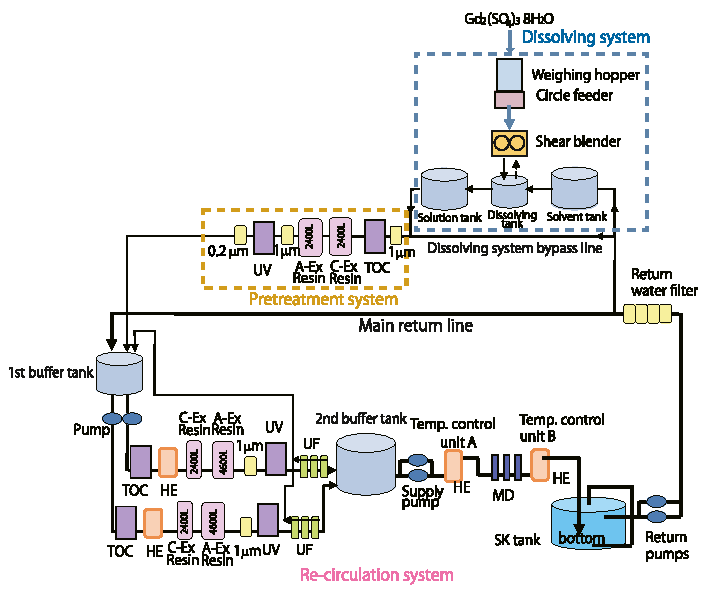
\includegraphics[width=15cm]{Figures/002/F13_Water}
	\caption[Schematic view of water purification system]{\label{002_F13_Water} Schematic view of water purification system~\cite{2022Abe}. The dissolving system and the pretreatment system are used during Gd loading, while the re-circulation system is used during both Gd loading and data taking.}
\end{figure}

\subsection{Air purification system}
\vs\hs Most of radioactive backgrounds come from radon, which is rich in the rock of the Kamioka mine.
To reduce radioactive backgrounds, radon in the air should be reduced as much as possible.\\
\hs Figure~\ref{002_F15_AirSeason} shows the typical radon concentration in the air at the SK over a year.
Radon concentration in the air of the mine is 2,000 - 3,000 Bq$/$m$^{\text{3}}$ during the warm season, from May to October, while the concentration is 100 - 300 Bq$/$m$^{\text{3}}$ in the cold season, from November to April.
This is because the airflow inside the mine changes depending on the temperature outside the mine.
To keep the concentration below 100 Bq$/$m$^{\text{3}}$ inside the experimental area, fresh air is continuously blown at a flow rate of 10 m$^{\text{3}}/$min from outside the mine (Radon Hut) to the experimental area through an air duct.
The flow rate makes the air pressure inside the experimental area higher than outside, minimizing the entry of the air outside the experimental area.
As a result, the concentration inside the experimental area is kept at 30 - 50 Bq$/$m$^{\text{3}}$ throughout the year, as shown in Figure~\ref{002_F15_AirSeason}.\\
\hs However, the radon concentration inside the experimental area is still too high for observations with low radioactive backgrounds.
Therefore, the fresh air is purified using the air purification system, then the purified air is supplied to the gap between the top of the SK tank and the water surface.
Figure~\ref{002_F14_Air} shows the schematic view of air purification system.
Each component of air purification system is described in Ref.~\cite{2015NakanoPhD}.
The residual radon concentration in the purified air is a few mBq$/$m$^{\text{3}}$.

\begin{figure}[h]
	\centering
	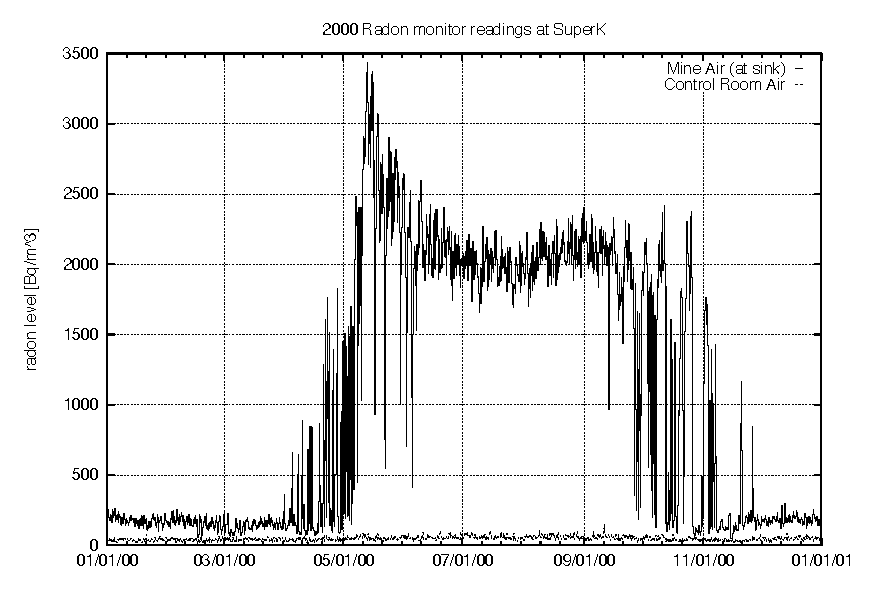
\includegraphics[width=12cm]{Figures/002/F15_AirSeason}
	\caption[Typical radon concentration in the air at the SK over a year]{\label{002_F15_AirSeason} Typical radon concentration in the air at the SK over a year~\cite{2003Fukuda}. The solid line shows the concentration outside the experimental area. The dashed line shows the concentration inside the experimental area.}
\end{figure}

\begin{figure}[tbp]
	\centering
	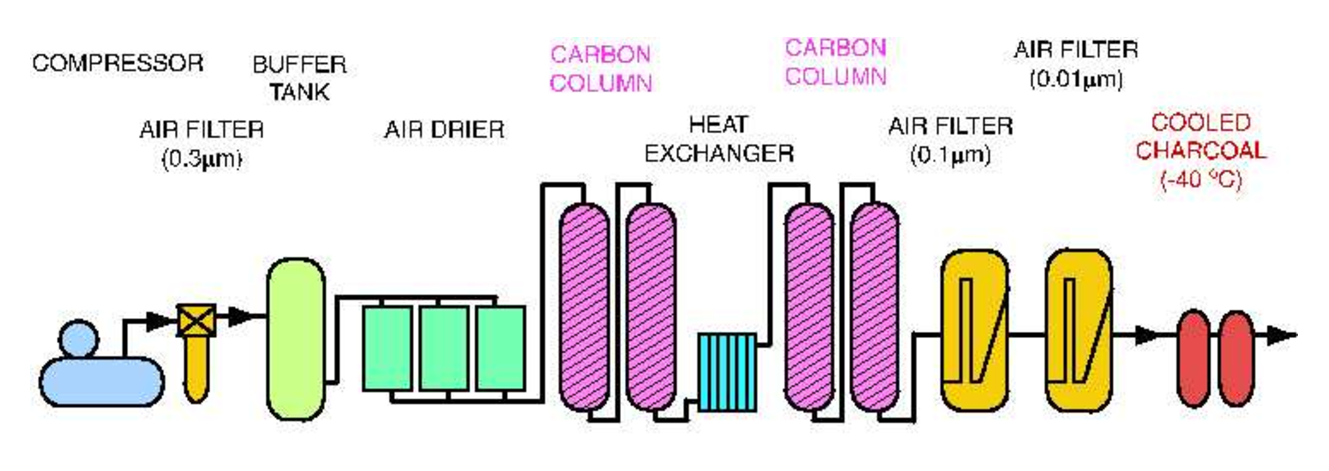
\includegraphics[width=15cm]{Figures/002/F14_Air}
	\caption[Schematic view of air purification system]{\label{002_F14_Air} Schematic view of air purification system~\cite{2003Fukuda}. Each component of air purification system is described in Ref.~\cite{2015NakanoPhD}.}
\end{figure}

\subsection{Data acquisition system}
\vs\hs As explained in Sec.~\ref{002_Obs_pha}, the data acquisition system was changed from ATM to QBEE in SK-IV.
The data used in this thesis was acquired by QBEE.
Therefore, the description of ATM is omitted in this thesis.\\
\hs Figure~\ref{002_F18_DAQ} shows the schematic view of the data acquisition system after SK-IV.
One QBEE board has 8 QTCs, and one QTC has 3 analog input channels for PMT signals.
That is, one QBEE board has 24 analog input channels for PMT signals.
Figure~\ref{002_F16_QTC} shows the block diagram of the QTC and its surroundings.
Each analog input channel has three gain ranges: small, medium, and large.
The gain ratio of small, medium, and large is set to 1, 1$/$7, and 1$/$49, respectively.
Also, the charge dynamic range of small, medium, and large is 0.2 - 51 pC, 1 - 357 pC, and 5 - 2500 pC, respectively.
The gain ratio is optimized to cover a wide charge dynamic range with reasonable resolution.
When the charge is sent to a QBEE board, the QTC integrates the charge and generates the output signal with the width proportional to the integrated charge.
Then the output signal is digitized by time-to-digital converter (TDC).
The digitized signals are transferred to 20 front-end PCs, and sent to 10 merger PCs.
In the merger PCs, the signals from all the front-end PCs are merged and the software trigger is applied.
Details about the software trigger is described later.
From the merger PCs, signals for triggered events are sent to an organizer PC and then written onto the disk for offline analysis.
Details about the front-end PCs, merger in the merger PCs, the organizer PC, and the disk are described in Ref.~\cite{2010Yamada}.

\begin{figure}[tbp]
	\centering
	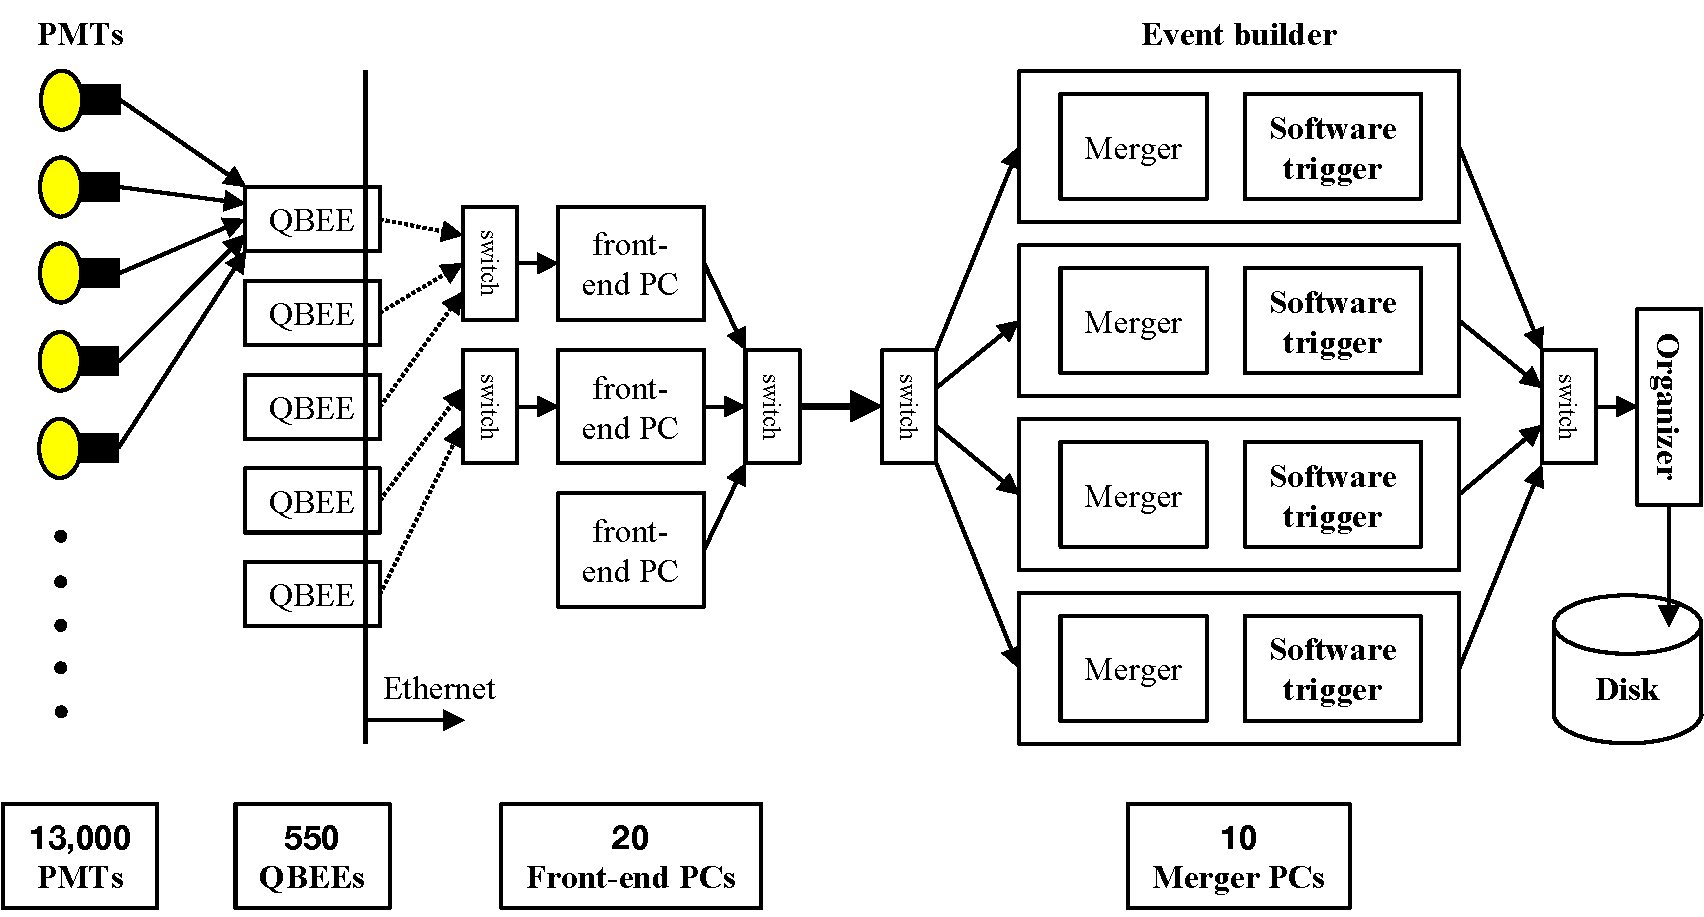
\includegraphics[width=15cm]{Figures/002/F18_DAQ}
	\caption[Schematic view of the data acquisition system]{\label{002_F18_DAQ} Schematic view of the data acquisition system~\cite{2010Yamada}.}
\end{figure}

\begin{figure}[tbp]
	\centering
	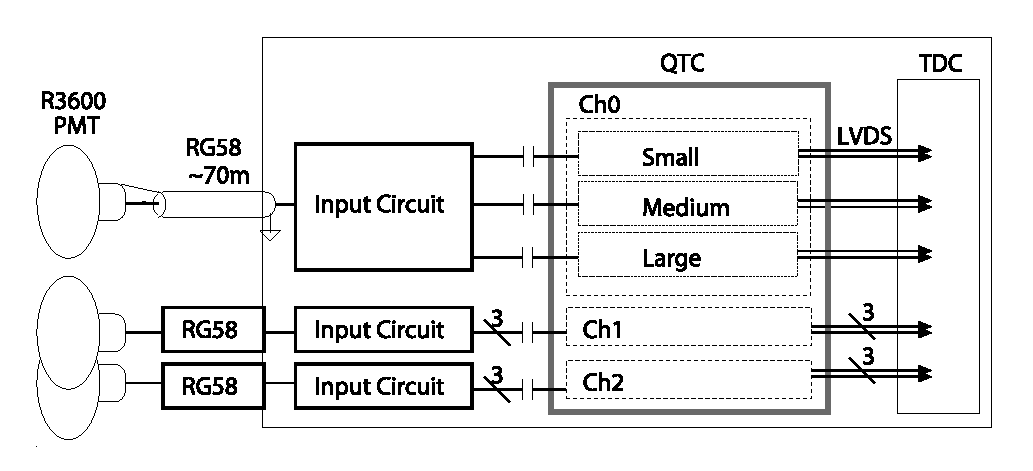
\includegraphics[width=15cm]{Figures/002/F16_QTC}
	\caption[Block diagram of the QTC and its surroundings]{\label{002_F16_QTC} Block diagram of the QTC and its surroundings~\cite{2009Nishino}. The output signal of each range (small, medium, or large) is generated by low voltage differential signaling (LVDS) drivers and digitized by time-to-digital converter (TDC).}
\end{figure}

\hs The software trigger process scans the signals sent to the merger PCs and searches the events satisfying the trigger conditions.
A trigger is applied when the number of ID PMT hits within 200 ns, which corresponds to the time that a Cherenkov photon moves from the edge of the SK tank to other, is a certain value or more.
Table~\ref{002_Tab:Tri} shows the trigger threshold and time width for recording PMT hits of each trigger type in SK-VI.
There are four trigger types for ID: Super Low Energy (SLE), Low Energy (LE), High Energy (HE), and Super High Energy (SHE).
Also, OD trigger is applied when the number of OD PMT hits within 200 ns is 22 or more.
Basically, when a trigger is applied, all hits from $-$5 $\mu$s to 35 $\mu$s are recorded, where the trigger timing is 0 $\mu$s.
However, in the case of SLE, all hits from $-$0.5 $\mu$s to 1.0 $\mu$s are recorded due to the high trigger rate.\\
\hs From SK-IV, a special trigger, AFT, was installed to search delayed neutron capture signals.
Previously, AFT trigger was applied when SHE trigger was applied and OD trigger was not applied to avoid the events by cosmic ray muons.
However, from SK-V, the condition about OD trigger was removed to study the spallation events by cosmic ray muons.
When AFT trigger is applied, all hits from 35 $\mu$s to 535 $\mu$s in addition to from $-$5 $\mu$s to 35 $\mu$s are recorded.

\begin{table}[tbp]
	\caption[Trigger threshold and time width for recording PMT hits of each trigger type in SK-VI]{\label{002_Tab:Tri} Trigger threshold and time width for recording PMT hits of each trigger type in SK-VI. $N_{\text{200, ID}}$ and $N_{\text{200, OD}}$ shows the number of ID or OD PMT hits within 200 ns.}
	\centering
	\vs
	\begin{tabular}{ccc}
		\hline\hline
		Trigger type&Trigger threshold&Time width [$\mu$s]\\
		\hline
		SLE&$N_{\text{200, ID}}\ge$ 34&1.5\\
		LE&$N_{\text{200, ID}}\ge$ 49&40\\
		HE&$N_{\text{200, ID}}\ge$ 52&40\\
		SHE&$N_{\text{200, ID}}\ge$ 60&40\\
		OD&$N_{\text{200, OD}}\ge$ 22&40\\
		\hline\hline
	\end{tabular}
\end{table}

%\begin{figure}[tbp]
%	\centering
%	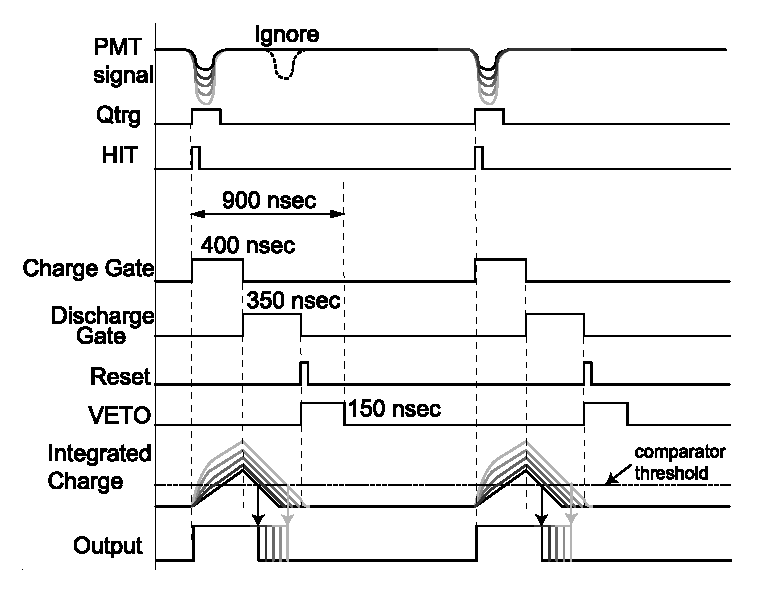
\includegraphics[width=12cm]{Figures/002/F17_QTCt}
%	\caption[Timing chart for QTC operation]{\label{002_F17_QTCt} Timing chart for QTC operation~\cite{2009Nishino}.}
%\end{figure}

\newpage
